% unicodeは、hyperrefへの指定で、pdfのメタデータにあるタイトルの文字化けを防ぐ
% ptは細かい指定はできないらしい
% A cheat sheet
% https://www.cpt.univ-mrs.fr/~masson/latex/Beamer-appearance-cheat-sheet.pdf
\documentclass[unicode, 14pt, aspectratio=169]{beamer}
\usetheme{titech}
\addbibresource{main.bib}
\date{\today}
\title{一貫性と可用性によるシステムの分類}
\author{\texttt{ryotaro612}}
\newcommand\blfootnote[1]{%
  \begingroup
  \renewcommand\thefootnote{}\footnote{#1}%
  \addtocounter{footnote}{-1}%
  \endgroup
}

\begin{document}
\begin{frame}[noframenumbering, plain]
\titlepage
\end{frame}
\section{Jepsen}
\begin{frame}
  \frametitle{Jepsen: 分散システムのテストフレームワーク\cite{jepsen}}
  {\large Jepsenはフォールトインジェクションに特化}
  \begin{itemize}
  \item Clojureのライブラリ
  \item テストケースは次のProtocolの実装
    \begin{itemize}
    \item 分散システムのクライアント
    \item 起こしたい障害
    \item クライアントの操作と障害のスケジュール
    \item 実行結果の確認
    \end{itemize}
  \item Jepsenに実装を呼出、実行結果の保存、再現をまかせる
  \end{itemize}
\end{frame}
\begin{frame}
  \frametitle{Jepsenの高い認知}
  {\large 今日までに45のストレージがテストされた\cite{jepsen-analysis}}
  \begin{itemize}
  \item テスト対象の抜粋
    \begin{itemize}
    \item etcd
    \item PostgresSQL
    \item MongoDB
    \item Elasticsearch
    \item Cassandra
    \end{itemize}
  \item テスト対象側のetcdからもJepsenへの言及がある\cite{jepsen-etcd}
  \end{itemize}
\end{frame}
\begin{frame}
  \frametitle{テスト対象を評価するときの課題}
  {\large 両立できる一貫性と可用性の強さを知ること}
  \par
  \vspace{8pt}
  CAP定理の問題
  \begin{itemize}
  \item CAP定理\cite{cap}の一貫性は線形化可能性\cite{linearizability}
  \item ほかの一貫性のモデルの参考にならない
  \item トリレンマではなく一貫性と可用性のトレードオフ\cite{cap-twelve-years-later}
    \begin{itemize}
    \item ネットワーク障害時に一貫性と可用性どちらを優先するかが問題
    \item 一貫性と可用性の選択は二者択一ではなく、複数の候補がある
    \end{itemize}
  \item 可用性の定義に矛盾した複数の定義がある\cite{kleppmann}    
  \end{itemize}
\end{frame}
\section{一貫性と可用性のパターン}
% \begin{frame}[t]
%   \frametitle{トレードオフの一貫性と可用性で比べる}
%   {\large 一貫性と可用性のペアは半順序関係になる}
% \end{frame}
\begin{frame}
  \frametitle{\normalsize{Highly Available Transactions Virtues and Limitations\cite{high}}}
  {\large 一貫性と両立できる可用性のペアを半順序関係に整理}
  \begin{columns}
    \begin{column}{0.5\textwidth}
      \begin{itemize}
      \item {\small 長さに上限のないネットワークの分断があることを前提}
      \item {\small ノードは一貫性を表現}
      \item {\small 枠の形状は可用性の種類を表現}
      \item {\small 楕円は実現できないペア}        
      \item {\small Jepsenに同様の図と一貫性の解説がある\cite{jepsen-models}}
      \end{itemize}
    \end{column}    
    \begin{column}{0.5\textwidth}
      \begin{figure}
        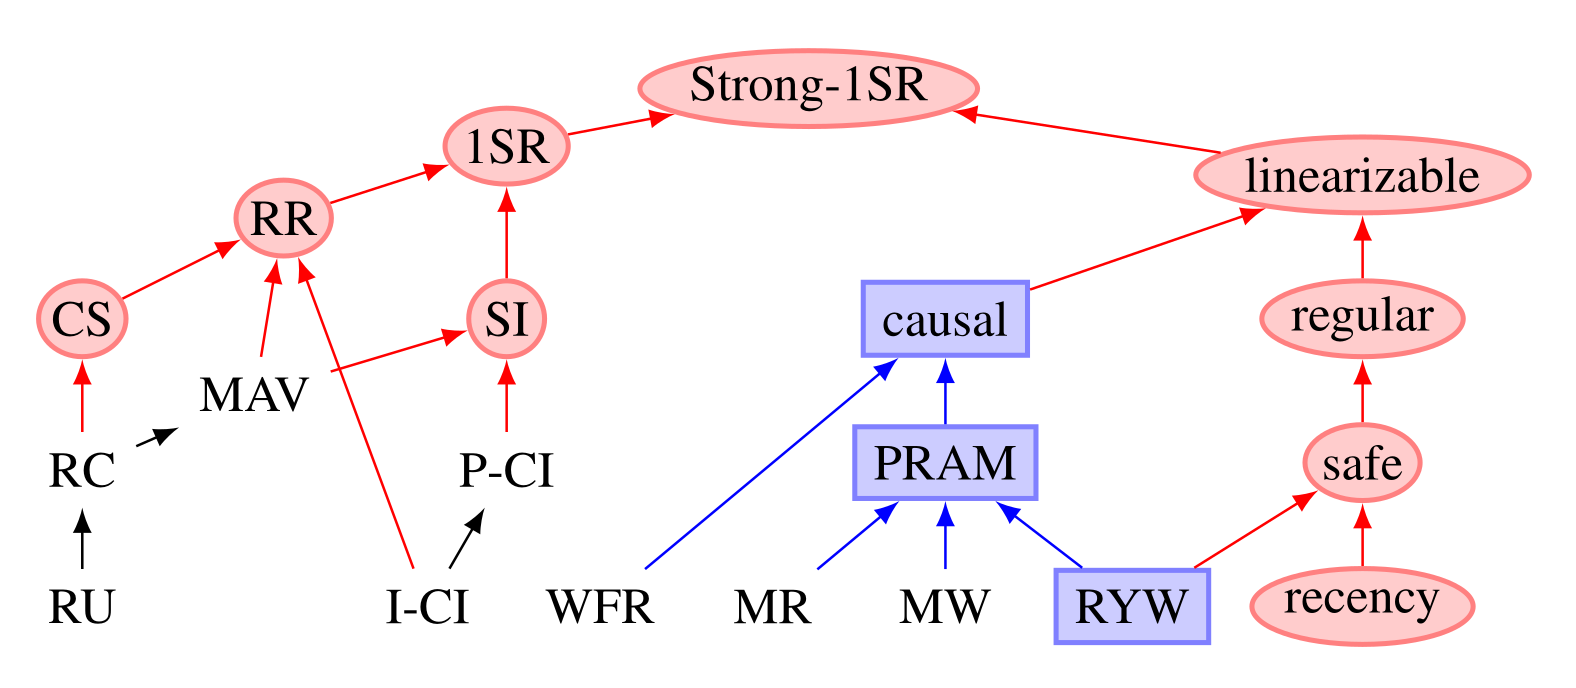
\includegraphics[width=1\textwidth]{images/hat.png}
        \caption{一貫性と可用性のペアの強さ\cite{high}}
      \end{figure}
    \end{column} 
  \end{columns}
\end{frame}
\begin{frame}
  \frametitle{2種類の可用性}
  {\large Sticky AvailabilityはHigh availablityの必要条件}
  \begin{description}
  \item[Sticky Availability] クライアントによる過去の全操作を反映したレプリカがあり、そのレプリカにトランザクションを実行するとき、クライアントに応答が返る
  \item[High Availability] すべてのクライアントがリクエストの送り先の正常なサーバから応答を受けとれる
  \end{description}
  どちら可用性も応答にかかる時間は問わない
\end{frame}
\begin{frame}
  \frametitle{くらべられるペアの例}
  {\large WFR, causal, linearizableは強さに関係がある}
  \begin{description}
  \item[WFR] プロセスがトランザクション$T_1$の後に$T_2$をコミットした場合に別のプロセスは$T_2$の結果を$T_1$の結果より先に参照できない
  \item[causal] すべてのプロセスが因果関係のあるの操作の同一な前後関係を観察していることを保証する。 一方、因果関係のない操作間はプロセスごとに異なる順序で観測されうる。
  \item[linearizable] 読み書き操作がアトミックであるように観測でき、かつ、すべてのプロセスの実行を仮に直列化したときと同じ実行結果になる
  \end{description}
\end{frame}
\begin{frame}[allowframebreaks,t]
  \frametitle{参考資料}
  \printbibliography
  \nocite{*}
\end{frame}
\end{document}
